\documentclass[11pt]{article}
\usepackage{geometry}                % See geometry.pdf to learn the layout options. There are lots.
\geometry{letterpaper}                   % ... or a4paper or a5paper or ... 
%\geometry{landscape}                % Activate for for rotated page geometry
%\usepackage[parfill]{parskip}    % Activate to begin paragraphs with an empty line rather than an indent
\usepackage{graphicx}
\usepackage{amssymb}
\usepackage{amsmath}
\usepackage{epstopdf}
\usepackage{hyperref}
\usepackage{natbib}
\DeclareGraphicsRule{.tif}{png}{.png}{`convert #1 `dirname #1`/`basename #1 .tif`.png}


\graphicspath{
}

\title{CTD-$\chi$pod Processing Guide}
\author{Andy Pickering}
%\date{}                                           % Activate to display a given date or no date


\begin{document}
\maketitle

\tableofcontents
\newpage


%~~~~~~~~~~~~~~~~~~~~~~~~~~~~~~~~~~~~~~
\section{Introduction}

This is a guide to processing data from CTD-$\chi$pods. $\chi$pods are self-contained instruments developed by the OSU Ocean Mixing Group to measure turbulence. They have a FP07 thermistor that measures temperature and temperature gradient, sampled at 100Hz. 

 
%~~~~~~~~~~~~~~~~~~~~~~~~~~~~~~~~~~~~~~
\section{Brief Outline of Major Processing Steps}

\begin{enumerate}
\item Find chipod data for each CTD cast
\item Align chipod data with CTD data
\item Calibrate chipod data
\item Apply chipod calc in 1 sec windows
\end{enumerate}
More details are given in the rest of the document.



%~~~~~~~~~~~~~~~~~~~~~~~~~~~~~~~~~~~~~~
\section{Software}
The processing is done with Matlab codes, which are maintained in a github repository: \newline
 \url{https://github.com/OceanMixingGroup/mixingsoftware}.\newline
  The CTD-$\chi$pod specific codes are in the folder \verb+/CTD_Chipod+. Codes for processing raw CTD data (.hex format) are contained in \verb+/ctd_processing+.



%~~~~~~~~~~~~~~~~~~~~~~~~~~~~~~~~~~~~~~
\section{Data Organziation}

Raw data should be organized into folders as:
\subsection{Raw Data}
\begin{itemize}
\item \verb+/Data/raw/Chipod/SNxxxx+ : Raw $\chi$pod data.
\item \verb+/Data/raw/CTD/+ : Raw CTD data (.hex,.XMLCON,.hdr).
\end{itemize}

Processed data is organized as follows:
\subsection{Processed Data}
\begin{itemize}

\item \verb+/Data/proc/Chipod/+ Main folder for processed $\chi$pod data

\item Data for each $\chi$pod is stored in \verb+/[whSN]/[pathstr]+ where \verb+pathstr+ constructed based on Params, for example:
\newline  \verb+zsm20m_fmax7Hz_respcorr0_fc_99hz_gamma20+
\newline
This allows us to run the processing for different Params and easily compare the results.

\item \verb+/Data/proc/CTD+ Processed CTD data. (/24Hz,/binned).
\end{itemize}


%~~~~~~~~~~~~~~~~~~~~~~~~~~~~~~~~~~~~~~
\section{CTD data}

CTD data needs to be obtained and processed before running the $\chi$pod processing.
Processing requires:
\begin{enumerate}
\item 24Hz data: used to determine the time offset between the CTD data and $\chi$pod data, by aligning (highpassed) dp/dt from the CTD with w estimated by integrating vertical chipod accelerations. 24Hz temperature is also used to calibrate the chipod temperature voltages and convert to physical units.
\item 1-m binned data: used to calibrate chi-pod T, and calculate dT/dz and $N^2$. 
\end{enumerate} 

I prefer to use codes in \verb+/mixingsoftware/ctd_processing/+ to process standard Seabird hex files into standard mat files to use in chi-pod processing. See \verb+Process_CTD_hex_Template.m+ for an example. The data can be processed using other methods, but must contain the specific fields required by the processing routines as listed below:

\subsection{24Hz CTD Data}

Required fields for 24Hz CTD data are:
\begin{itemize}
\item  dnum : datenum
\item t : temperature [C]
\item p : pressure [db]
\end{itemize}

\subsection{1-m Binned CTD Data}
Required fields for binned CTD data
\begin{itemize}
\item dnum : datenum
\item t : temperature [C]
\item p : pressure [db]
\item s : salinity [psu]
\item lat : Latitude [$^o$]
\item lon : Longitude [$^o$]
\end{itemize}



%~~~~~~~~~~~~~~~~~~~~~~~~~~~~~~~~~~~~~~
\section{Processing steps}

All templates are located in \verb+/mixingsoftware/CTD_Chipod/Templates/+

\begin{enumerate}

\item Modify \verb+Load_chipod_paths_template.m+ . This specifies filepaths to raw data, as well as where output will be saved.

\item Modify \verb+Chipod_Deploy_Info_template.m+ with info for specific deployment. Much of the rest of the processing uses information from the above two files.

\item Plot the raw chi-pod data (\verb+Plot_Raw_Data_template+?). This will let you see quickly if any sensors or files are obviously bad. If there are bad files you can specify these in a \verb+Bad_File�+  list so they will not be loaded during processing (this is not necessary, but will reduce time loading bad files, and may prevent bad data from accidentally being used).  Figure \ref{x} shows an example of a normal-looking file. Figure \ref{xx} shows an example of file that looks bad.

\item  Modify \verb+MakeCasts_CTDchipod_Template.m+ for specific cruise. This script finds $\chi$pod data for each cast, aligns the data, calibrates the data, and saves a file with data for each cast. 

\item  Run \verb+MakeCasts_CTDchipod+ for one good cast for each SN. Check time-offset / alignment; if not right, probably need to modify \verb+az_correction+ or switch AX and AZ. Figure \ref{x} shows an example of where AX and AZ are flipped.  * figures showing example of flipped ax etc*

\item  Once that is figured out, run \verb+MakeCasts_CTDchipod+ for all casts. Data are saved to \verb+/Data/proc/Chipod/cast+ and \verb+/Data/proc/Chipod/cal+.

\item Run \verb+SummarizeProc_Template+. This makes some summary tables and figures from the `Xproc.mat' data saved during  \verb+MakeCasts_CTDchipod+.

\item \verb+Plot_TP_profiles_EachCast_Template.m+ For each cast, this plots the temperature derivative from all chi pod sensors on the same scale so you can compare them and check for bad profiles. Figures are save to \verb+/Figures/TPprofiles/+

\item  Modify \verb+DoChiCalc_Template.m+ and run for all casts. This does the chi calculation for all the cast files made in \verb+MakeCasts_CTDchipod+. Data are saved to  \verb+/Data/proc/Chipod/avg/+

\item \verb+Make_Combined_Chi_Struct_Template+

\item \verb+PlotXCsummaries_Template+. Make summary plots

\end{enumerate}



%~~~~~~~~~~~~~~~~~~~~~~~~~~~~~~~~~~~~~~
\section{$\chi$pod Processing Parameters}

Variable parameters for the processing are specified in a `Params' structure.

\begin{itemize}
\item fmax : Maximum frequency to integrate temperature gradient spectrum to (default 7 Hz).
\item gamma : Assumed mixing efficiency (default 0.2).
\item \verb+resp_corr+ : Option to apply frequency response correction (default 0).
\item fc : Cutoff frequency for response correction (if applied) (default 99 for naming purposes).
\item \verb+z_smooth+ : The distance [m] over which $N^2$ and $dT/dz$ are smoothed (default 10m).
\end{itemize}



%~~~~~~~~~~~~~~~~~~~~~~~~~~~~~~~~~~~~~~
\section{Output File Formats}

%~~~~~~~~
\subsection{/cast}
`Raw' (ie uncalibrated) $\chi$pod data for each cast. Structure `cast' with fields:
\begin{itemize}
\item datenum
\item T1 = Temperature [V]
\item T1P - dT/dt [V]
\item AX - X-acceleration [V]
\item AZ - Z-acceleration [V]
\item \verb+chi_files+ - List of raw chipod files from which data was combined into this structure.
\item \verb+time_range+ - Time range of CTD cast.
\item castname - Name of CTD cast.
\end{itemize}
Ex. filename : \verb++

%~~~~~~~~
\subsection{/cal}
Calibrated data for each cast. Up and down casts are saved in separate files. Structure `C' with fields:
\begin{itemize}
\item datenum
\item P [db]
\item T1P - dT/dt [Ks^{-1}]
\item fspd - [ms^{-1}]
\item castidr - up/down
\item info
\item ctd
\end{itemize}
Ex. filename : \verb+rh10011_SN2013_downcast.mat+

%~~~~~~~~
\subsection{/avg}
Result of $\chi$pod calculations. Contains data points for each 1 sec window.
\begin{itemize}
\item Params
\item datenum
\item  P - [db]
\item N2 - 
\item dTdz
\item fspd - [ms^{-1}]
\item T [^oC]
\item S [psu]
\item theta
\item sigma
\item chi1- $\chi$ []
\item eps1 $\epsilon$ []
\item KT1 $K_T$ []
\item TP1var
\item samplerate - [hz]
\item nu
\item tdif
\item lat
\item lon
\item castname
\item castdir
\item Info
\end{itemize}
Ex. filename : \verb+avg_08402_downcast_SN1013_T1.mat+


%~~~~~~~~~~~~~~~~~~~~~~~~~~~~~~~~~~~~~~
\section{Notes}

There is a template for standard latex notes that can be modified for each cruise/deployment: \verb+Chipod_Notes_Template_AP+.

%The following scripts/functions make some standard tables and plots for the notes.
%\verb+SummarizeProc_Template.m+
%\verb+PlotXCsummaries_Template.m+
%\verb+MakeTableChiDeploy.m+


%~~~~~~~~~~~~~~~~~~~~~~~~~~~~~~~~~~~~~~
\section{Post-processing Analysis}

\begin{itemize}
\item Plot $\chi$pod time-offsets. The time-offset should drift linearly with time, and may be reset during the cruise. Typically should be less than 20 sec (depends on how accurately time was set). In some cases, the time was set wrong (off by a day, wrong time zone etc.); in this case the processing script needs to be modified to correct this.
\item Compare different sensors and cast directions: The quality of data obtained depends heavily on the setup of the CTD and the $\chi$pod mounting. Typically the upward looking sensors on the upcasts are the cleanest data. 
\item Sensitivity to parameters: see details below.
\end{itemize}



%~~~~~~~~~~~~~~~~~~~~~~~~~~~~~~~~~~~~~~
\section{Sensitivity Analysis}

The sensitivity of the results to different parameters should be examined, including \verb+fmax+ and \verb+z_smooth+.

\verb++



%~~~~~~~~~~~~~~~~~~~~~~~~~~~~~~~~~~~~~~
\section{Standard Plots made by processing}

\begin{itemize}
\item \verb+cast_001_RawChipodTS+ (Figure \ref{tsraw}).

\item \verb+cast_001_w_dTdtSpectraCheck+ (Figure \ref{speccheck}). This compares the analog $dT/dt$ (T1P) to the differentiated T signal. The spectral amplitudes should agree up to a certain frequency where the digital dT/dt becomes dominated by noise. If the spectra below the noise level don't match, the time-constant used in calibration might need to be modified. 

\item \verb+cast_001_w_TimeOffset+ (Figure \ref{align})

\item \verb+cast_001_w_TimeOffset_Zoom+ (Figure \ref{alignzoom}). Shows a zoomed-in period of the time-offset. The two timeseries should match in the lower panel. 

\item \verb+cast_001_T_P_dTdz_fspd+ (Figure \ref{tscal}). Summary of the alilgned and calibrated data.

\item \verb+cast_001_upcast_chi_SN600_T1_avg_chi_KT_dTdz+ (Figure \ref{avgsum}). Summary of the final data (`avg' structure).

\end{itemize}


\clearpage
\newpage
%~~~~~~~~~~~~~~~~~~~~~~~~~~~~~~
\section{Example Figures}


\begin{figure}[s]
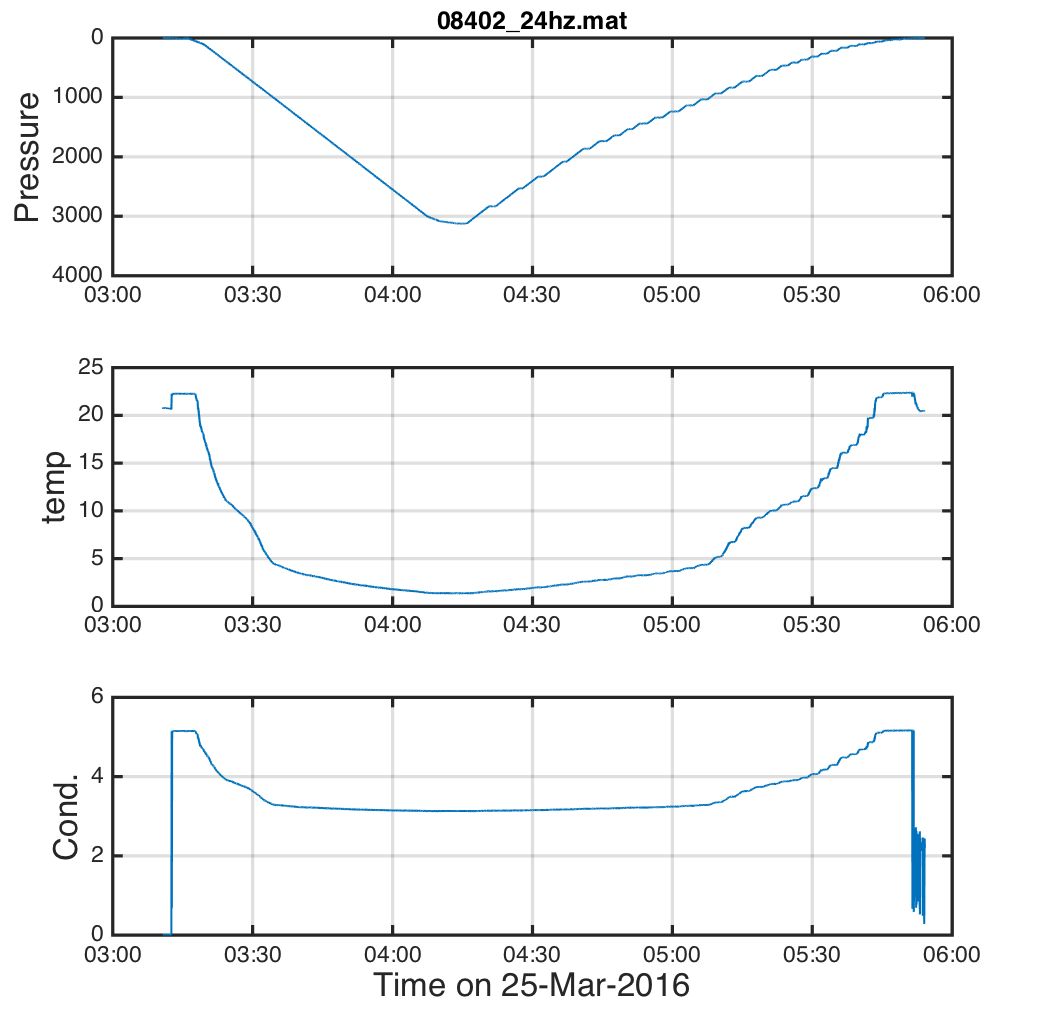
\includegraphics[scale=0.75]{SN1013_08402_Fig0_RawCTD.png}
\caption{Time-series of raw CTD data for one cast.}
\label{ctdraw}
\end{figure}


\begin{figure}[s]
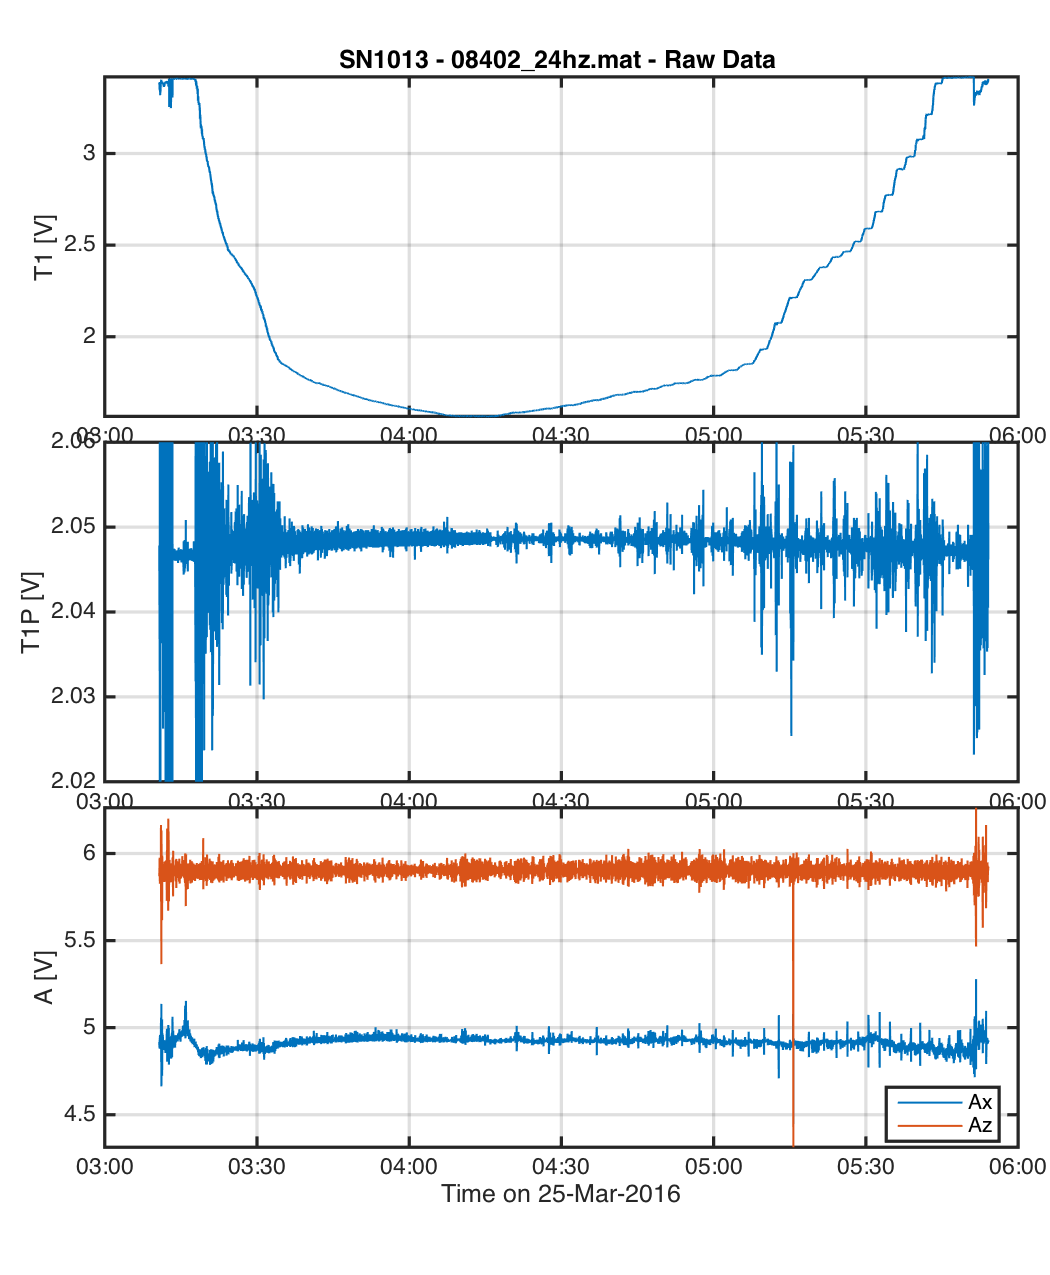
\includegraphics[scale=0.75]{SN1013_08402_Fig1_RawChipodTS.png}
\caption{Time-series of raw $\chi$pod data for one cast.}
\label{tsraw}
\end{figure}

\begin{figure}[s]
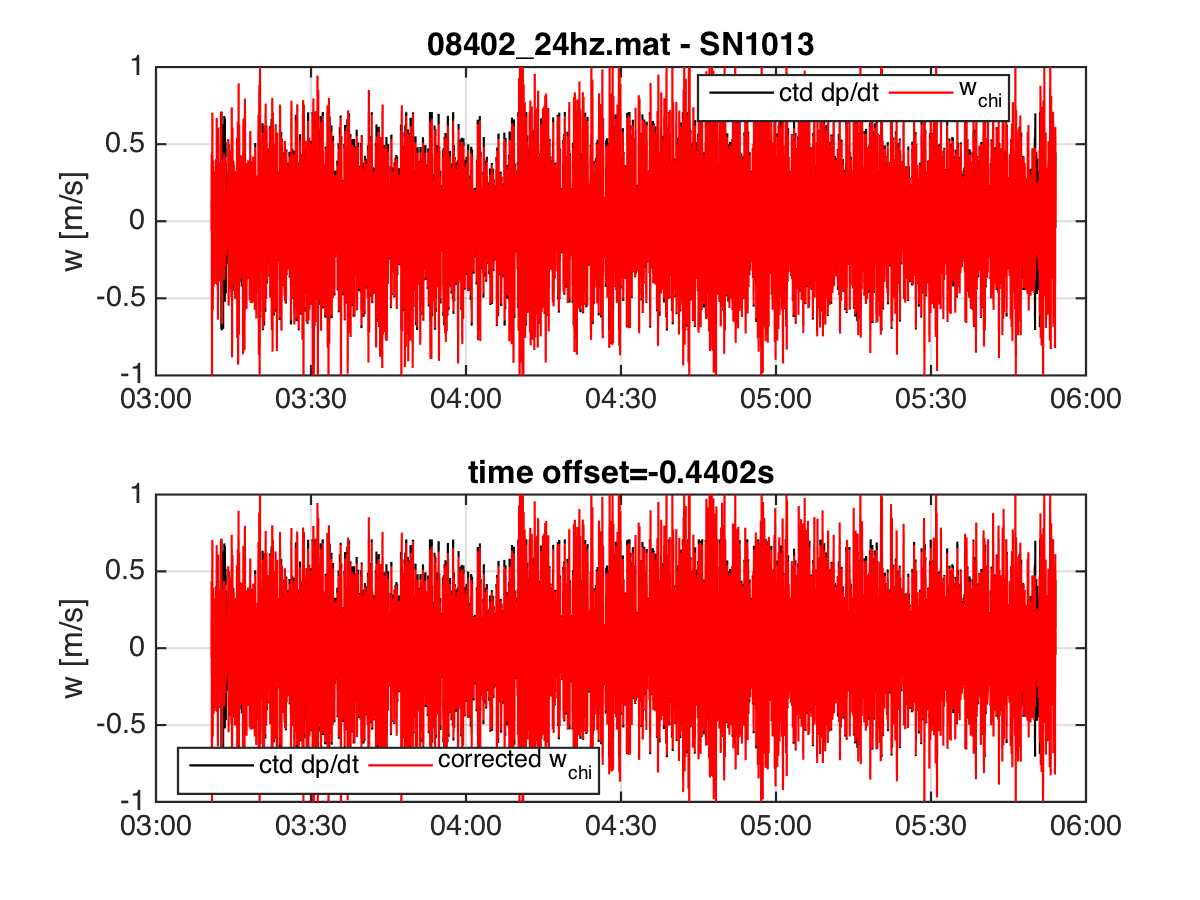
\includegraphics[scale=0.75]{SN1013_08402_Fig2_w_TimeOffset.png}
\caption{Time series of dp/dt CTD and chipod w. Top is original, bottom is after time-offset applied to chipod.}
\label{align}
\end{figure}

\begin{figure}[s]
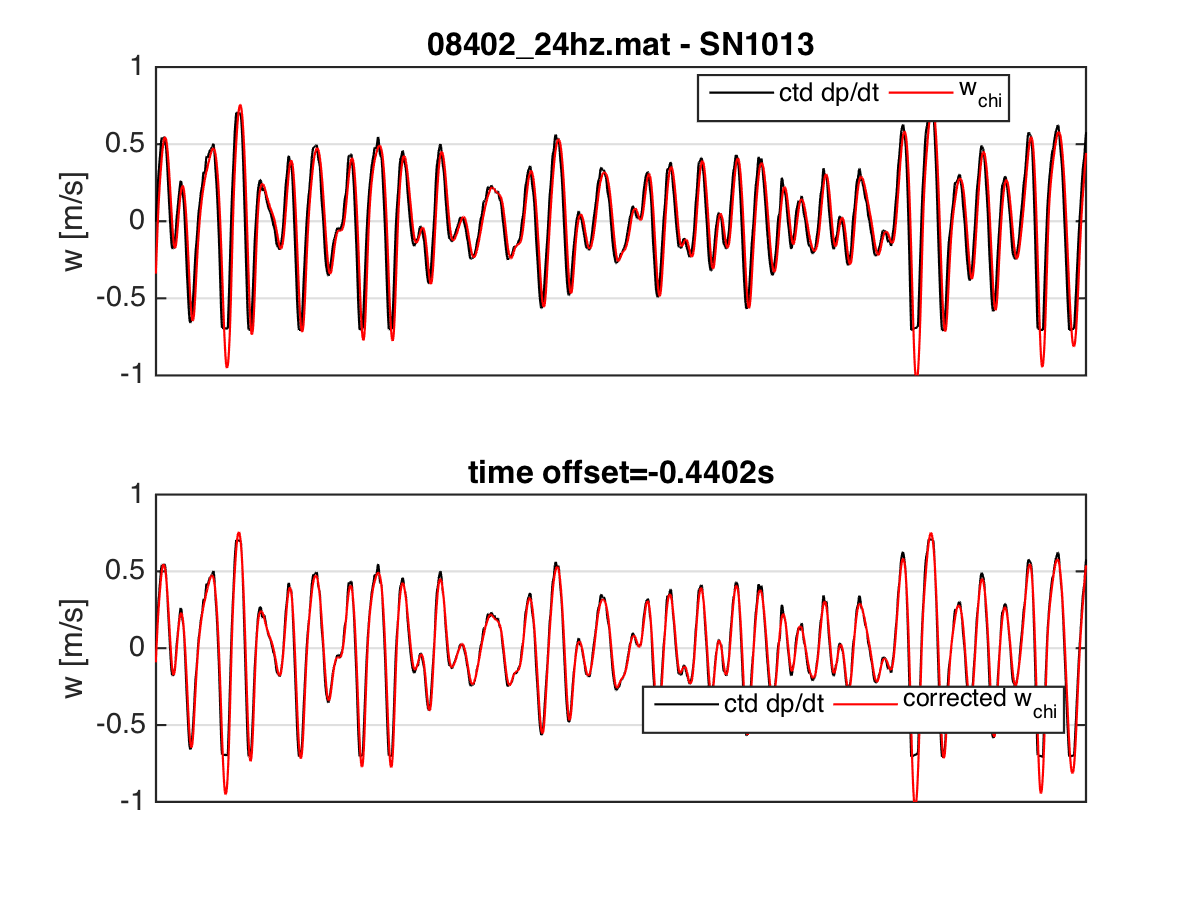
\includegraphics[scale=0.75]{SN1013_08402_Fig3_w_TimeOffset_Zoom.png}
\caption{Zoom-in of dp/dt and chipod w allowing one to check if time-offset is correct. Bottom panel should match.}
\label{alignzoom}
\end{figure}

\begin{figure}[s]
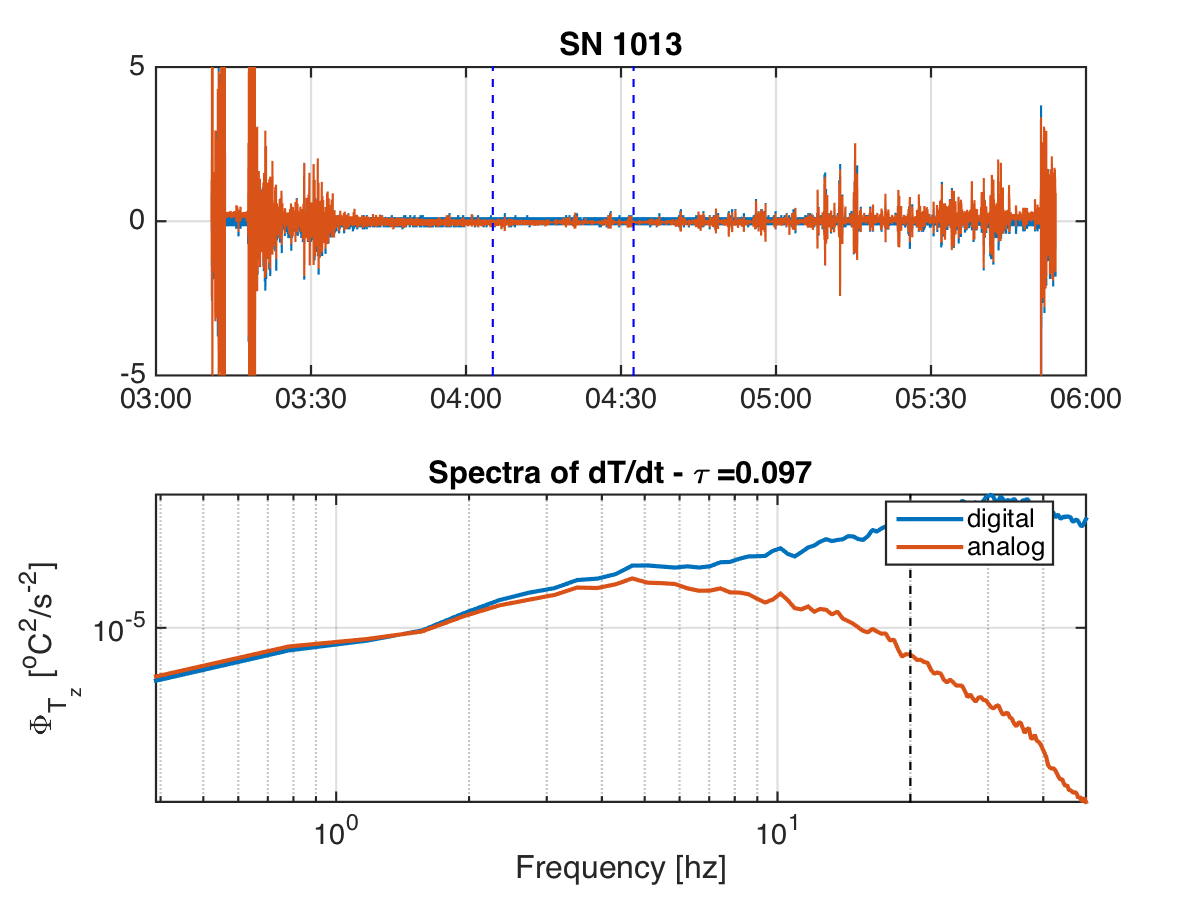
\includegraphics[scale=0.75]{SN1013_08402_Fig4_dTdtSpectraCheck.png}
\caption{dT/dt spectra for analog (TP) and digital derivatives. Spectra levels should match; if not time-constant may be wrong.}
\label{speccheck}
\end{figure}


\begin{figure}[s]
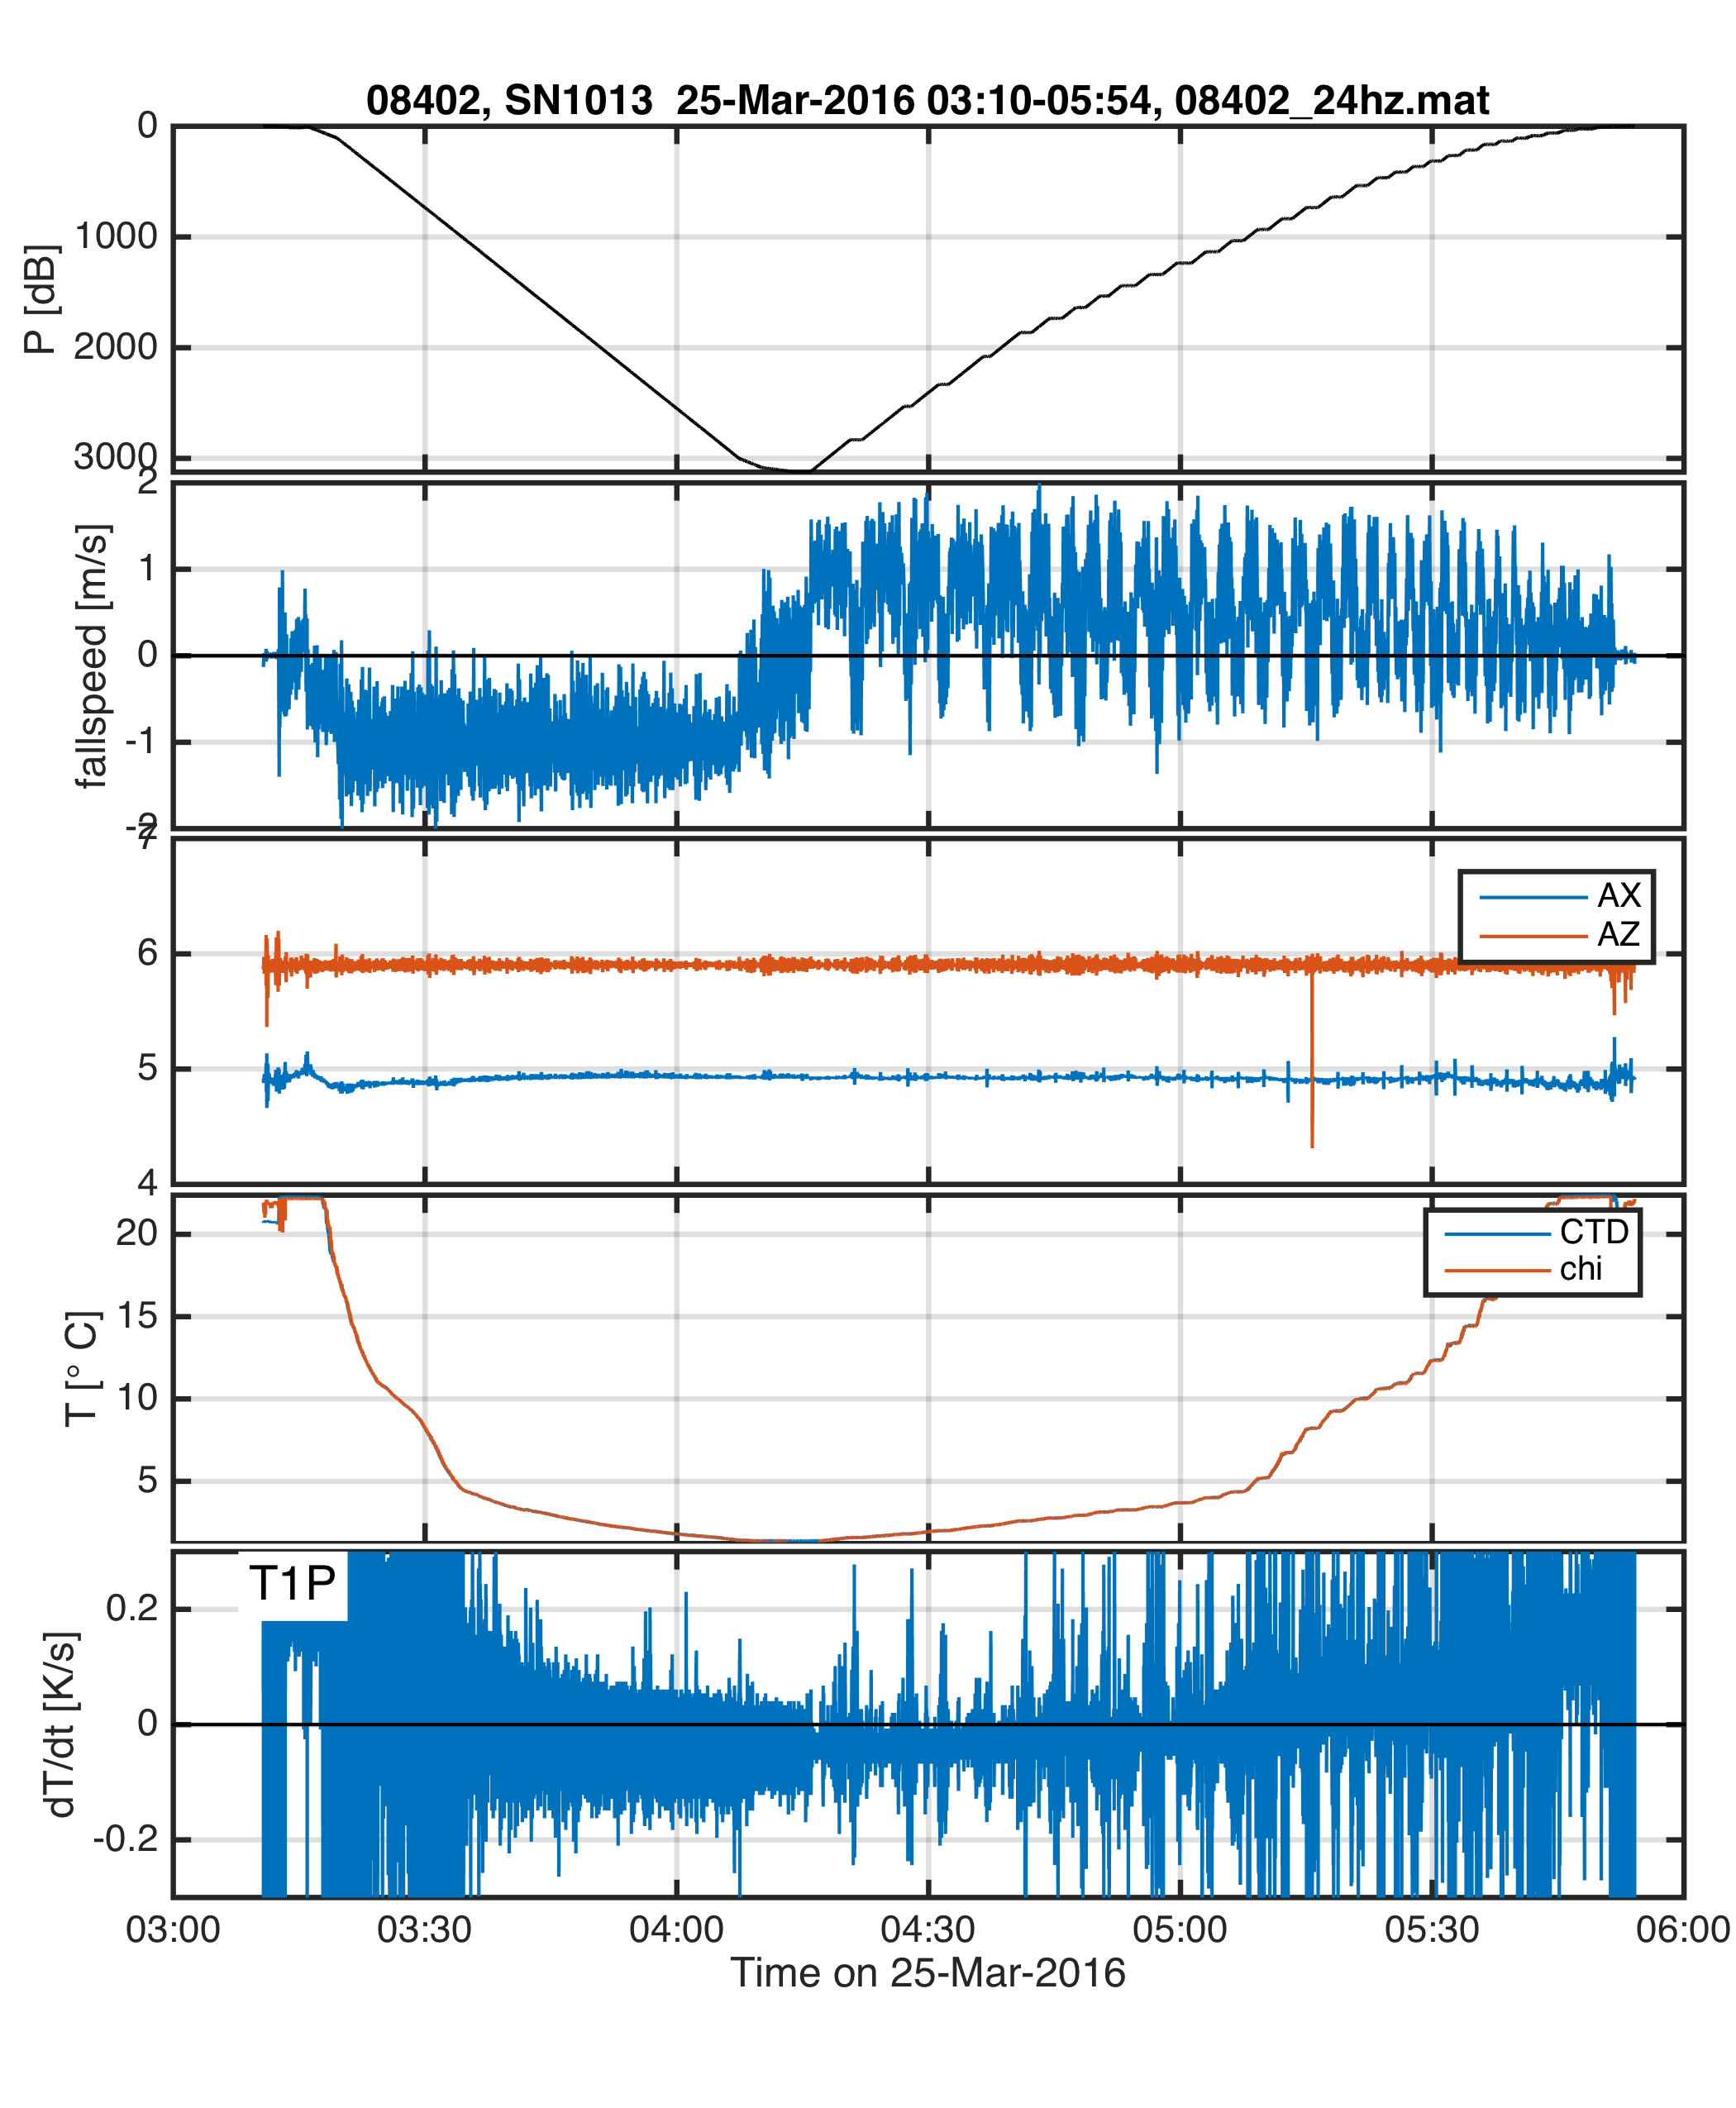
\includegraphics[scale=0.75]{SN1013_08402_Fig5_T_P_dTdz_fspd.png}
\caption{Time series of aligned and calibrated chipod data for one cast.}
\label{tscal}
\end{figure}


\begin{figure}[s]
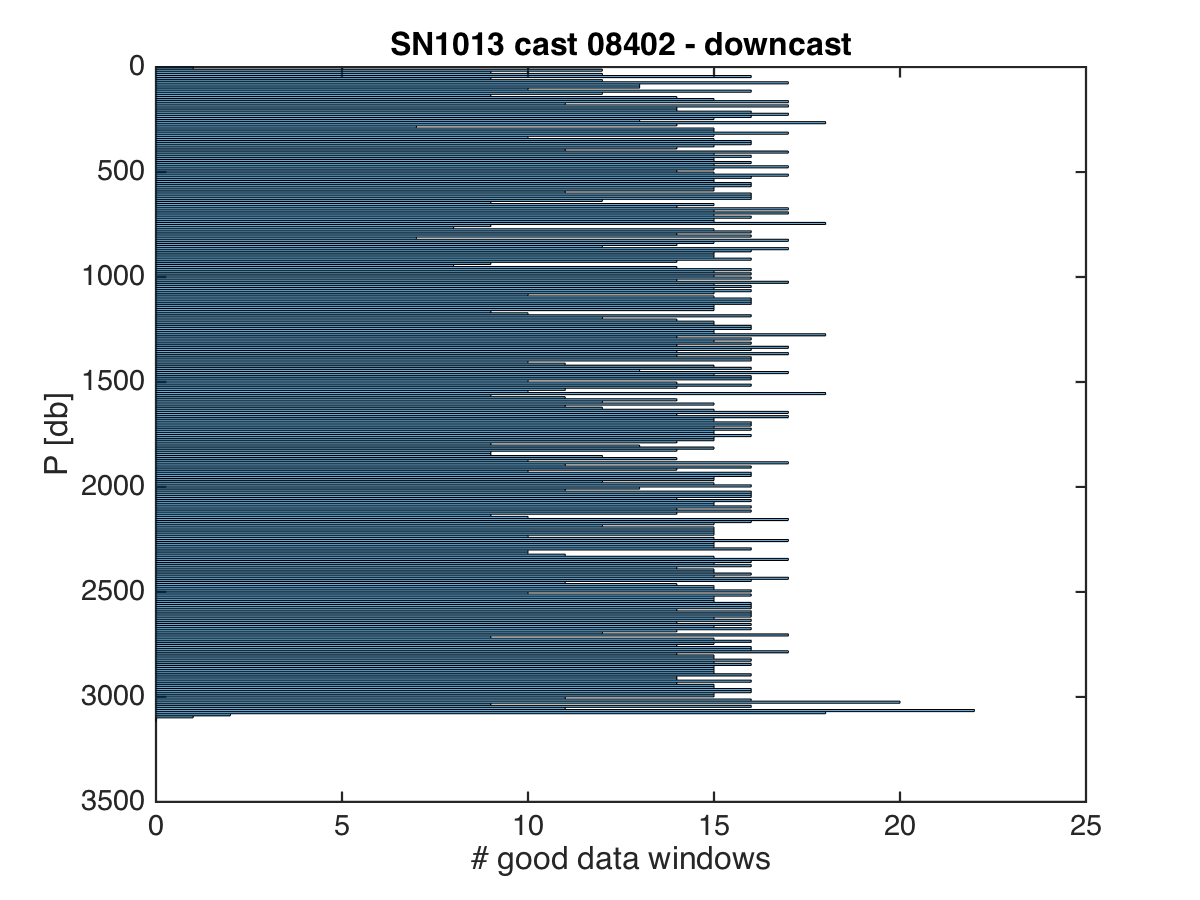
\includegraphics[scale=0.75]{SN1013_08402_Fig6_downcast_chi_T1_avgPhist.png}
\caption{Histogram of the number of good $\chi$pod data windows in each 10m depth bin.}
\label{histgood}
\end{figure}


\begin{figure}[s]
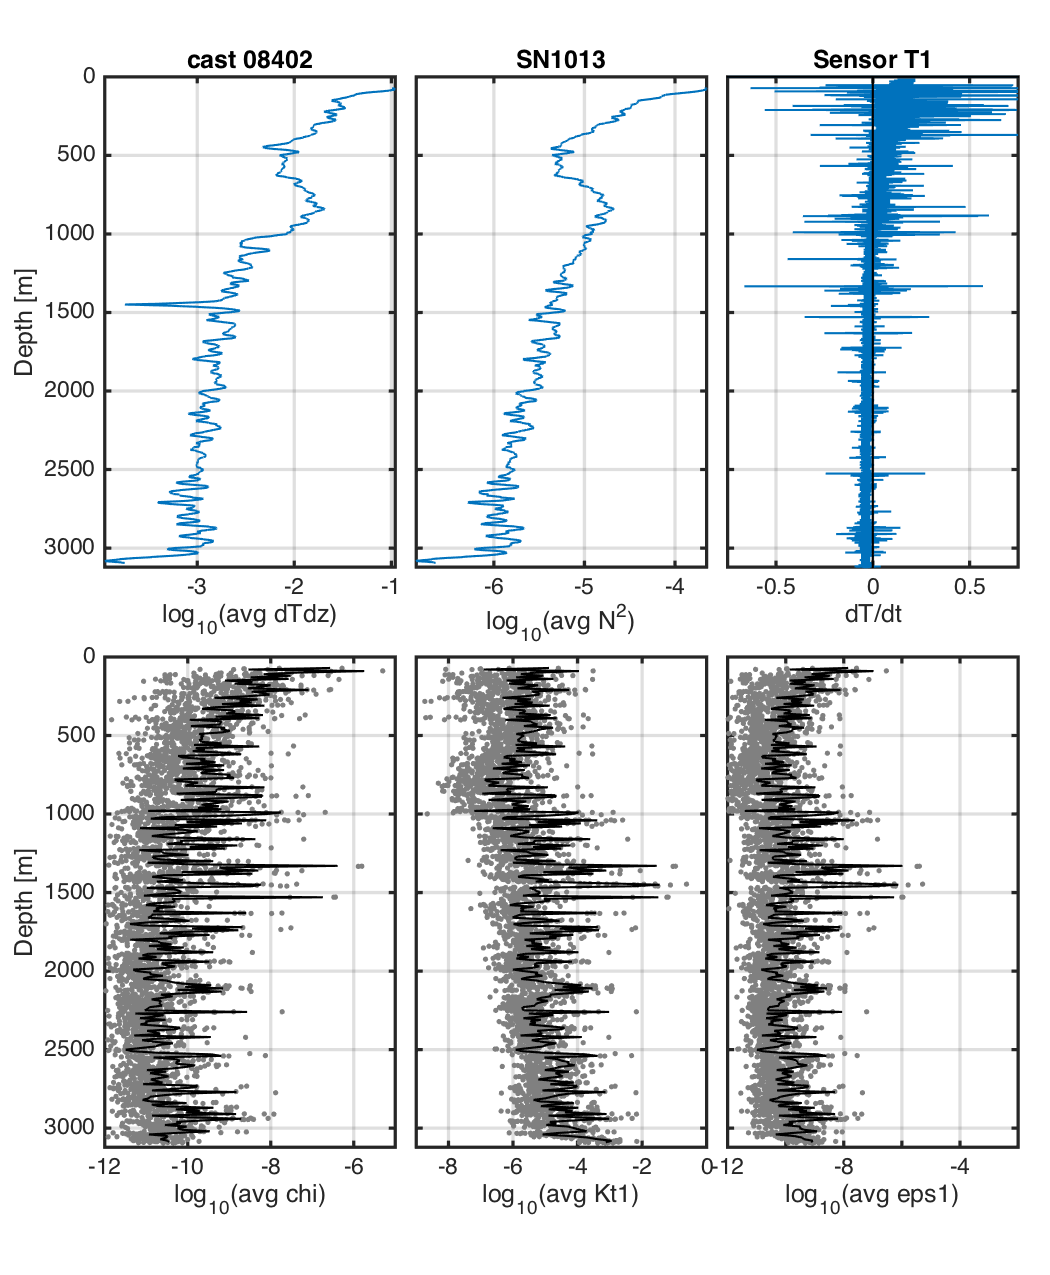
\includegraphics[scale=0.75]{SN1013_08402_Fig7_upcast_chi_T1_avg_chi_KT_dTdz.png}
\caption{Results of chipod calculation for one cast. Black lines in lower panel are 10m binned averages.}
\label{avgsum}
\end{figure}



\clearpage
\newpage
%~~~~~~~~~~~~~~~~~~~~~~~~~~~~~~~~~~~~~~
\section{m-files}

Processing files are kept in a GitHub repository \verb+/mixingsoftware/CTD_Chipod/mfiles/+

\begin{itemize}
\item \verb+AlignChipodCTD+ : Align CTD and chipod data.
\item \verb+Compute_N2_dTdz_forChi+
\item \verb+get_chipod_chi+ : Main function that does chipod calculation.
\item \verb+load_chipod_data+
\item \verb+MakeCtdChiWindows+
\item \verb++
\end{itemize}



%~~~~~~~~~~~~~~~~~~~~~~~~~
 \bibliographystyle{ametsoc2014}
\bibliography{/Users/Andy/Cruises_Research/wavechasers_bib/main}




\end{document}  
